% !TeX root = ../diss.tex

\chapter{Evaluation}
I performed two investigations to evaluate my work; to find out whether my implementations were correct, and their performance characteristics.

\section{Correctness testing}
\label{sec:Correctness_eval}

I tested whether my designs would correctly align sequences as I produced them.
After developing each implementation, I thoroughly tested it to ensure that it would produce a correct and optimal alignment for any pair of sequences.
I did this to stop errors from being carried over from one implementation to the next, as outlined in \cref{sec:Methodology_prep}.

Each implementation needs to produce alignments that are correct and optimal.
A correct alignment will produce two strings which are substrings of the input sequences, after gap symbols (\lstinline{-}) are removed from the alignment sequences.
An optimal alignment will have the highest score of any of the possible alignments between the sequences.
There can be multiple optimal alignments, with the same score, when the \lstinline{max} functions in the implementations choose different pointers when the argument of the \lstinline{max} functions have the same value (\cref{sec:SW_DP}).

I used the alignment program in EMBOSS \cite{EMBOSS} to test my C implementation, and then used my C implementation to test my CUDA and SystemVerilog implementations.
I used EMBOSS to find the scores of optimal alignments between sequences and checked my program produced an alignment with the same score.
My C implementation would also check if alignments were valid, and this code was checked against the substring checker built into Python.

To test the CUDA and SystemVerilog implementations, the C program was used to check the scores of the alignments, and to check that the alignments were valid.
A small set of test sequences was also used during the development process, especially when simulating the SystemVerilog, but each implementation was tested thoroughly when I finished working on it.

This was the testing approach applied to a large set of test sequences. Many of the sequences were randomly generated from lengths $1$ to $\SI{131072}{}$, and others were specific edge cases (such as identical sequence pairs, or pairs with no shared characters).
I also used the set of proteins that relate to humans or mice in SwissProt database \cite{UniProt}; a total of $\SI{37393}{}$ sequences ranging in length from $2$ to $\SI{35213}{}$ symbols. Approximately $\SI{100000}{}$ pairs of sequences were tested for each implementation.

No issues were found in the last correctness testing run for each of my implementations, thus I believe all three correctly and optimally align sequences.

\section{Performance testing}
\label{sec:Performance_eval}

\subsection{Testing approach}
\label{sec:Performance_approach}

I also tested the performance of my different implementations, mainly by measuring the amount of time they took to align sequences, comparing the implementations and different variants of the same implementation.
DNA and protein sequence datasets based on real-world data were not ideal for testing sequence alignment programs.
DNA datasets tend to be made up of very long sequences (often significant fractions of a chromosome, which are made up of hundreds of thousands if not millions of symbols), and the protein dataset SwissProt \cite{UniProt} did not have sequences of the lengths I wanted to test against.

Instead, I produced a synthetic dataset to evaluate my program.
I resampled the distribution of amino acids in proteins in humans \cite{AminoAcidFreqs} to produce protein sequences, and I resampled the distribution of codons (trigrams of nucleotides) \cite{CodonFreqs} to produce DNA sequences.
This meant they were similar to true sequences, and because they were randomly generated pairings were unlikely to form edge cases in alignments.

\subsubsection{Testing environment}
\label{sec:Testing_environment}
All tests were run on my Dell XPS 15 9570 laptop, running Ubuntu 18.04 LTS.
It has an Intel i7-8750H CPU, an Nvidia GTX 1050 Ti GPU, and 16 GB of DDR4 RAM.

Each performance test was run $10$ times, and the averages are plotted in the figures, with error bars of $\pm\sigma$.
For several figures, this interval is very small and the error bars are occluded by the point markers.
When sampling $10$ times, this $\pm\sigma$ error bar provides a $99.84\%$ confidence interval if the samples are normally distributed.
Trendlines are linear unless otherwise stated.

\subsection{Comparing implementations}
\label{sec:Comparing_implementations}

Comparisons between all three implementations are limited by the SystemVerilog implementation, which can only align sequence pairs shorter than $1024\times1536$.
\Cref{fig:All3} shows the throughput of each implementation (the average amount of time taken to align a pair of sequences), in milliseconds.
Using increased parallelism and specialisation, the FPGA is able to significantly outperform the CPU and GPU for shorter sequences.

For short sequences, not as many threads are required, so the better single-threaded performance of the CPU dominates over the GPU.
However, when evaluating against long sequences, the GPU implementation is able to use increased parallelism to outperform the CPU.
\Cref{fig:All3_Big} shows the throughput when aligning a sequence of length $\SI{32768}{}$ against the given length.

Also included on \cref{fig:All3_Big} is an extrapolated speed for the FPGA, using the formula derived in \cref{sec:Processing_time_on_FPGA}, with the result doubled.
The design I produced was space limited, but only the most expensive FPGAs have enough embedded memory to align these long sequences with the quadratic space algorithm.
Instead, a linear space approach is required, doubling the amount of arithmetic required, so \cref{fig:All3_Big} plots double the value given by the formula in \cref{sec:Processing_time_on_FPGA}.
This is only a rough estimate, an actual design is likely to have a different number of processing elements and clock speed to my quadratic space design.

Using this approximation, there is a small difference between the FPGA and GPU.
Although the FPGA design is highly specialised, the clock speed is much lower than the GPU and only allows for $48$ concurrent cell evaluations, whereas the GPU can execute $768$ threads simultaneously.
This comparison is not completely fair due to the age difference between the devices (\cref{sec:FPGA_prep}), and a newer and larger FPGA might be able to perform significantly better than the GPU.

\begin{figure}[H]
    \centering
    \begin{subfigure}{.49\textwidth}
      \centering
      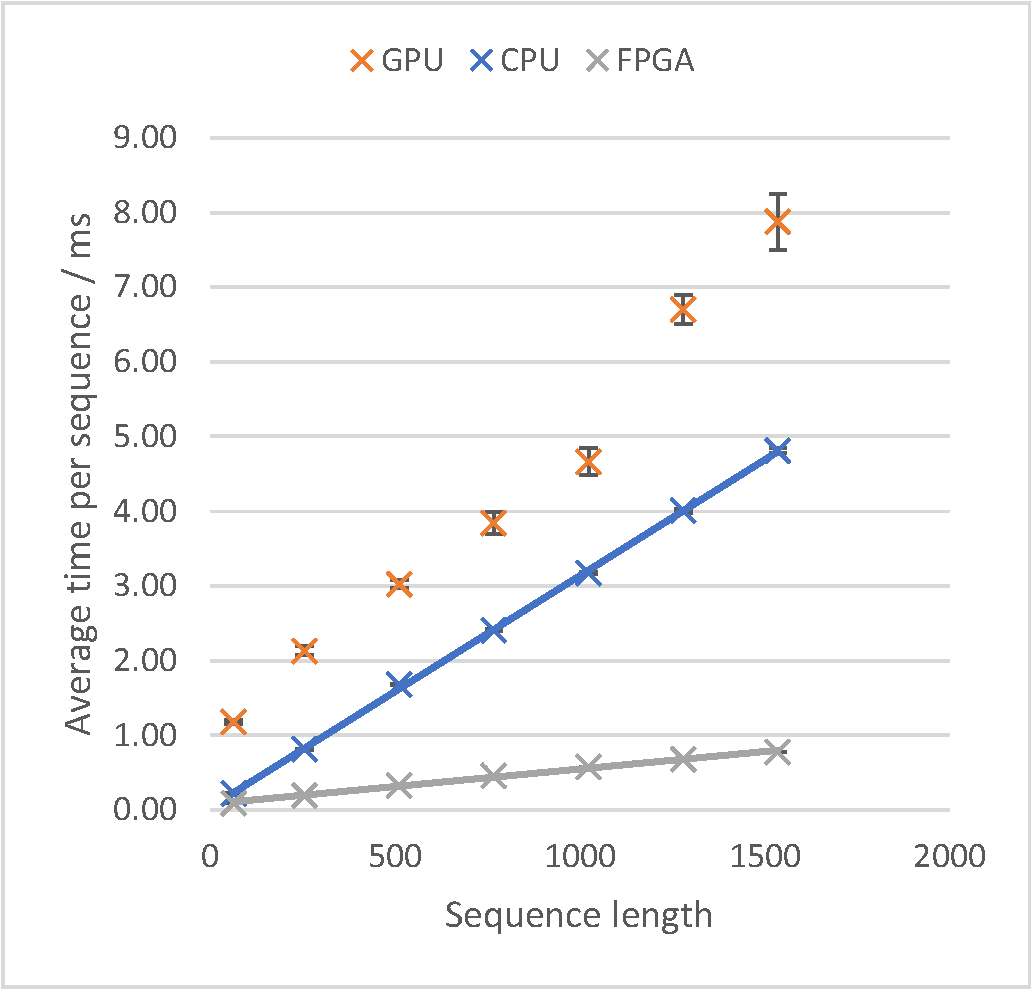
\includegraphics[width=\linewidth]{figs/eval/all3_blosum.pdf}
      \caption{Aligning two proteins using BLOSUM50 \mbox{substitution} matrix. CPU: $R^2=0.9997$, FPGA:~${R^2=0.9957}$}
      \label{fig:All3_BLOSUM}
    \end{subfigure}%
    \hfill
    \begin{subfigure}{.49\textwidth}
      \centering
      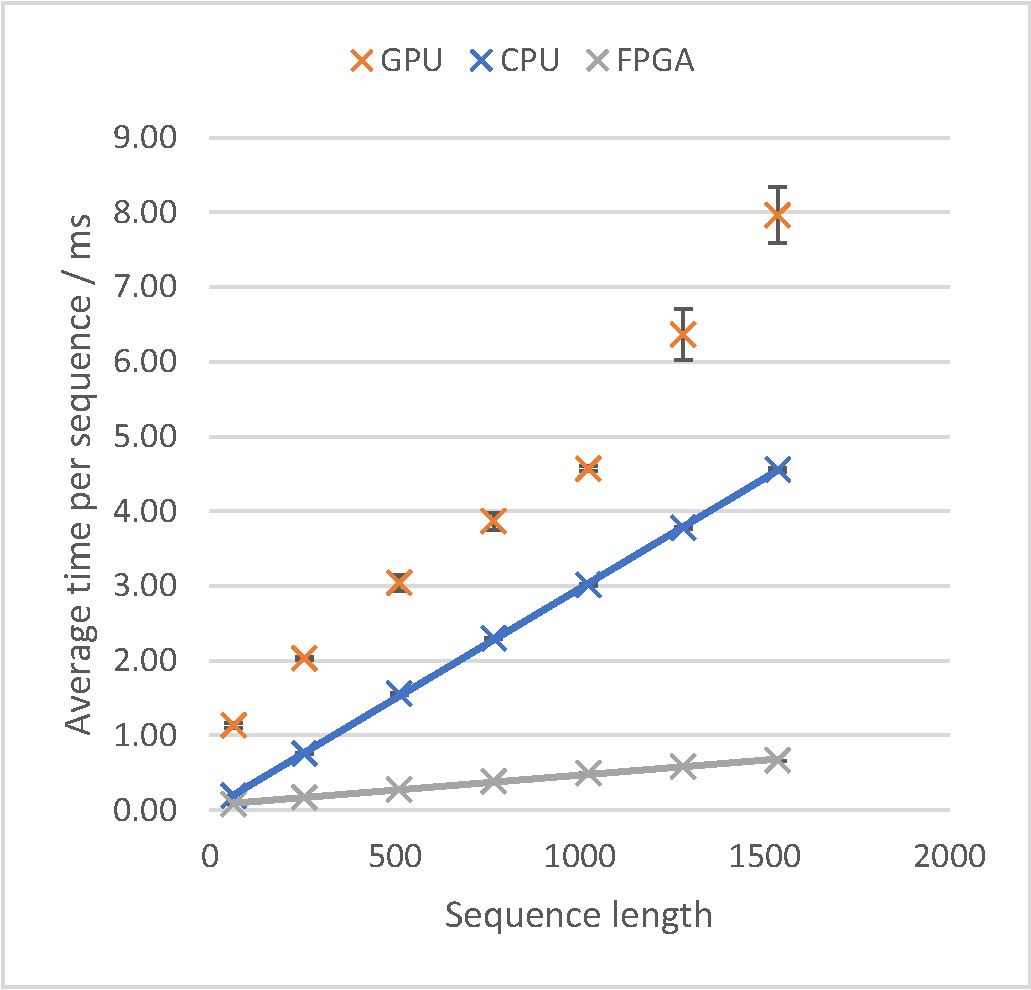
\includegraphics[width=\linewidth]{figs/eval/all3_dna.pdf}
      \caption{Aligning two DNA sequences using a constant similarity function. CPU: $R^2=0.9999$, FPGA:~${R^2=0.9967}$}
      \label{fig:All3_DNA}
    \end{subfigure}
    \caption{Throughput of aligning a sequence of length $1024$ against the given length}
    \label{fig:All3}
\end{figure}

\begin{figure}[H]
    \centering
    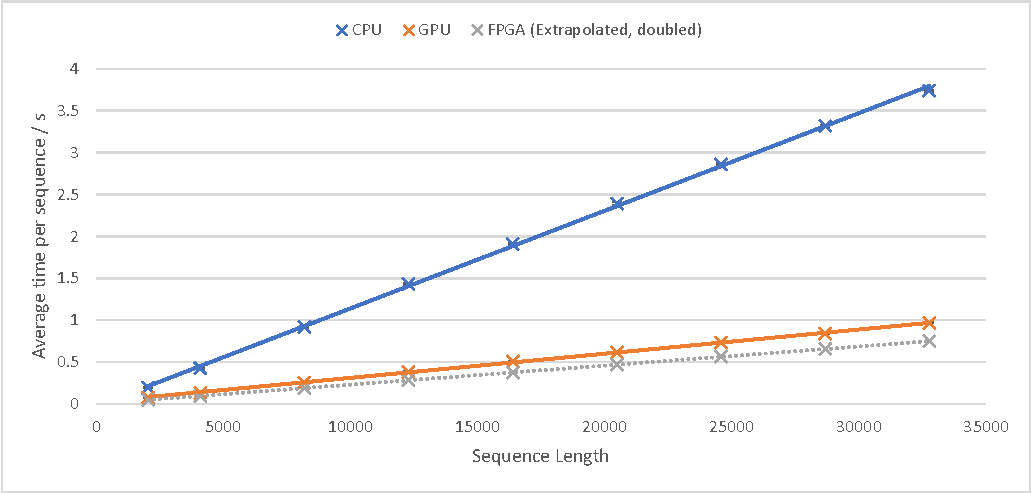
\includegraphics[width=\textwidth]{figs/eval/all3_big.pdf}
    \caption{Throughput of aligning two proteins of length $\SI{32768}{}$ against the given length, using BLOSUM. CPU: $R^2=0.9995$, GPU: ${R^2=0.9994}$}
    \label{fig:All3_Big}
\end{figure}

\subsection{C implementation}
\label{sec:C_eval}

\subsubsection{Setting implementation parameters}
\label{sec:C_params_eval}

The first tests were to set the implementation parameters, values that change how the program performs but do not change the output.
One parameter is the point at which the linear space program has sufficiently subdivided the alignment and calls the quadratic space program instead.
To set this crossover point, a set of $12$ alignments of two $\SI{32768}{}$-symbol long sequences of proteins were performed by the parallel linear space implementation, with the crossover length set at different points.
The impact of this (which can be seen in \cref{fig:C_Crossover}) was minor, but smaller crossover points appeared to be slightly better so I used a crossover value of $1024$ symbols.
Setting the value below $1024$ led to instability due to the number of threads required.

\begin{figure}[H]
    \centering
    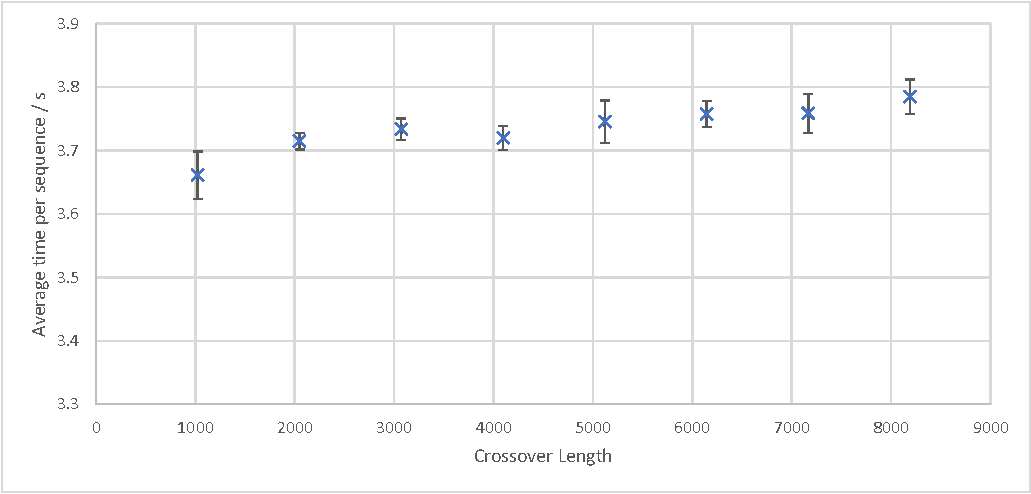
\includegraphics[width=\textwidth]{figs/eval/c_crossover.pdf}
    \caption{Throughput of aligning two proteins both of length $\SI{32768}{}$, using BLOSUM, at different crossover points. Note the y-axis starts at $\SI{3.3}{\s}$.}
    \label{fig:C_Crossover}
\end{figure}

The other parameter to consider was the number of threads that could be working at one time, which was controlled using a semaphore (\cref{sec:Multi_threaded_C_impl}).
This was tested by measuring the time it took to align $24$ pairs of proteins of lengths $\SI{32768}{}$, and turned out to be a demonstration of simultaneous multithreading, and the results are shown in \cref{fig:C_Cores}.

There were no significant speedups when allowing more than $6$ threads to work, but this did very gradually speed up till $12$ threads.
However, the amount of time spent by threads resident in the CPU (user time) increased nearly linearly until $12$ threads.
Up to $12$ threads can be resident in a 6-core CPU with Intel's Hyperthreading technology (thus the linear increase in user time) but there are only enough resources in a core for an average of one thread's work to be done (thus the minor changes in wall time).
The minor decrease in wall time between $6$ and $12$ threads (between $\SI{4.13}{\s}$ and $\SI{3.56}{\s}$ respectively) is probably due to the two threads occasionally being able to share resources on the CPU, extracting a $16\%$ speedup.
Based on this information, I chose to run my tests with up to $12$ threads working at one time.

\begin{figure}
    \centering
    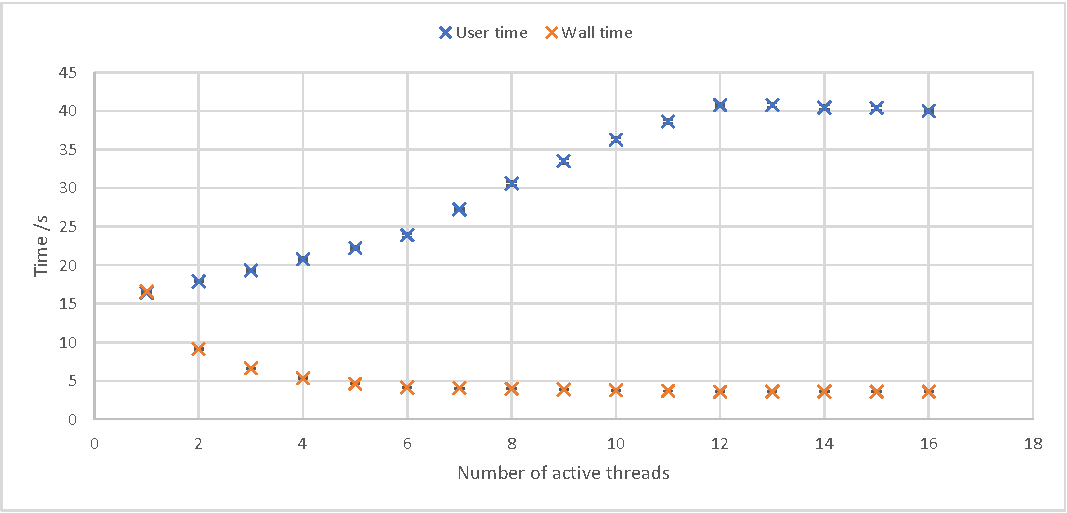
\includegraphics[width=\textwidth]{figs/eval/c_cores.pdf}
    \caption{Time taken to aligning $24$ pairs of proteins both of length $\SI{32768}{}$, using BLOSUM, using different numbers of cores}
    \label{fig:C_Cores}
\end{figure}

\subsubsection{Quadratic, Linear Space, and Multithreaded implementations}
\label{sec:C_impls_eval}

Two metrics to compare the different implementations in C are latency and throughput.
Throughput measures the average time spent on each sequence, whereas latency measures the time between starting and finishing an alignment.
\Cref{fig:C_Space_IL} shows the throughput of the different implementations, measured by allowing up to $12$ threads to work on a set of alignments.
The linear space algorithms will use the quadratic space algorithm to align sub-sequences shorter than $1024$ symbols, though significant differences are not seen until aligning sequences of lengths $\SI{16384}{}$ and $\SI{32768}{}$ symbols.
One reason for this divergence is decreasing parallelism for the quadratic space algorithm as the space requirements grew, because fewer alignments could happen at the same time due to lack of memory.

In \cref{fig:C_Space_IL} the linear parallel implementation can use more than one thread to perform an alignment, whereas the simple linear version only uses one thread per alignment.
The number of threads used by an alignment does not affect throughput because the total amount of work done by the processor is the same, even if it can be distributed differently.
However, there is an impact on latency as shown in \cref{fig:C_Space_Ser}.

Latency was measured by sequentially aligning a set of sequences, as opposed to multiple sequences being aligned at a time when measuring throughput.
This is shown in \cref{fig:C_Space_Ser} and the parallelised implementation performs the best, because it recruits more than one CPU core.
The linear space variant involves double the arithmetic of the quadratic variant (\cref{sec:SW_Linear_Complexity}) yet only takes approximately $1.38$ times more time, likely due to less memory contention.
The parallel version was $2.41$ times faster than the linear space algorithm, compared to a maximum of $3$ times faster that could be expected (\cref{sec:Multi_threaded_C_impl}).

\begin{figure}
    \centering
    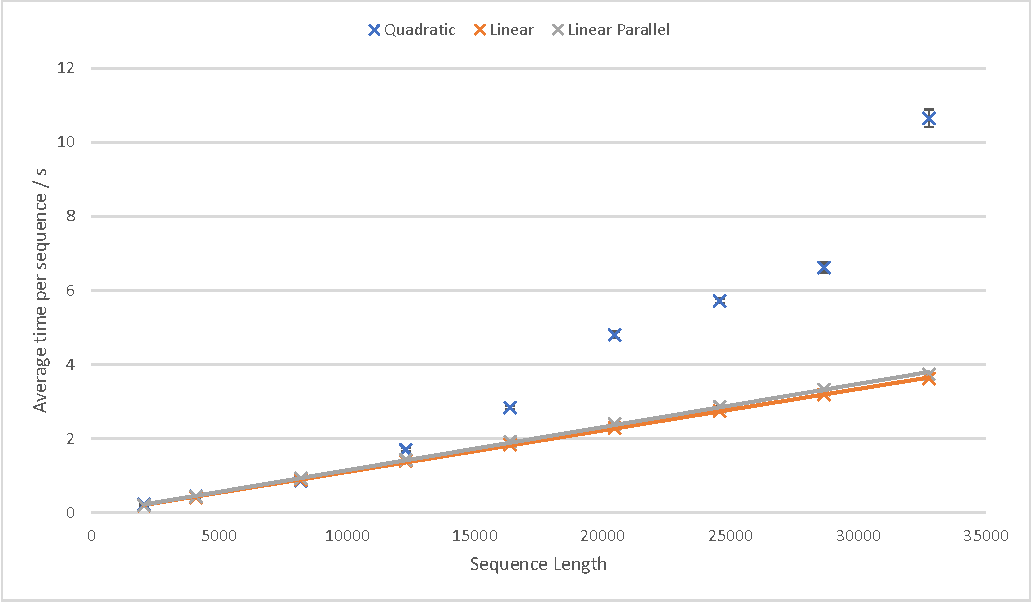
\includegraphics[width=\textwidth]{figs/eval/c_spaces_il.pdf}
    \caption{Throughput of aligning two proteins of length $\SI{32768}{}$ against the given length, using BLOSUM, using different C implementations. Linear: $R^2=0.9997$, linear parallel:~${R^2=0.9995}$}
    \label{fig:C_Space_IL}
\end{figure}

\begin{figure}
    \centering
    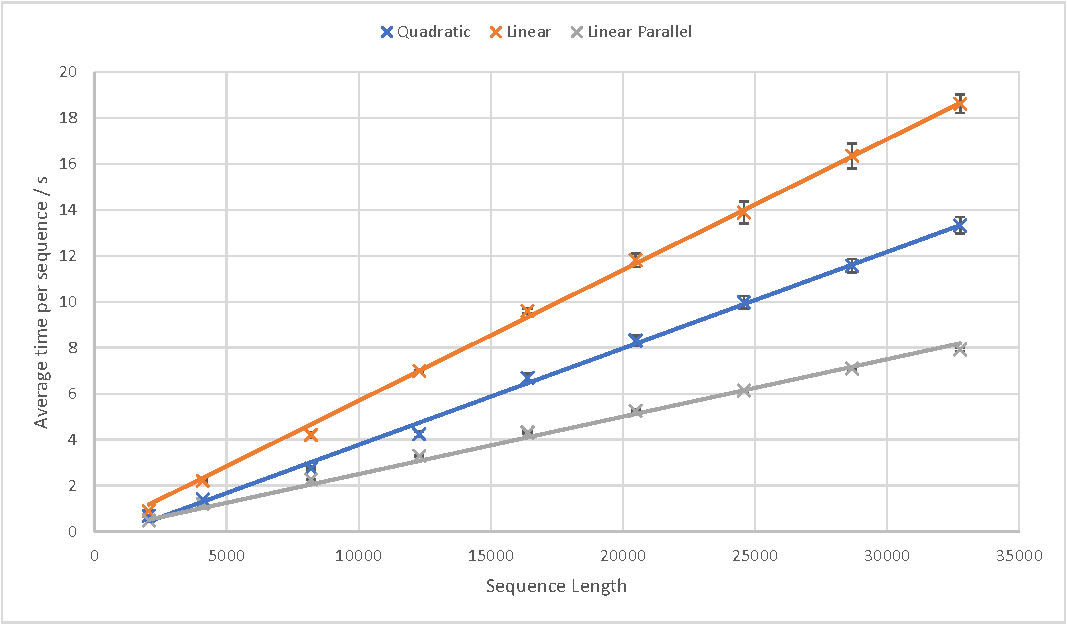
\includegraphics[width=\textwidth]{figs/eval/c_spaces_ser.pdf}
    \caption{Latency of aligning two proteins of length $\SI{32768}{}$ against the given length, using BLOSUM, using different C implementations. Quadratic: $R^2=0.9987$, linear: $R^2=0.9972$, linear parallel:~${R^2=0.9950}$}
    \label{fig:C_Space_Ser}
\end{figure}

\subsubsection{Sequence similarity functions and scoring gaps}
\label{sec:C_scoring_eval}

The impact of different methods of scoring methods (\cref{sec:SW_similarity_functions}) was also investigated; shown in \cref{fig:C_similarity_fun}.
I expected the gap between a constant function for proteins and BLOSUM, due to the cost of looking up values in the BLOSUM matrix.
I did not expect to see a gap between DNA and Protein constant functions, but this was likely due to differences in lengths of alignment for the different sets of sequences.
Interestingly, different results are found on the GPU (\cref{sec:CUDA_scoring_eval}).

The impact of different gap scoring methods (\cref{sec:SW_gaps}) was investigated; shown in \cref{fig:C_Gotoh}.
The extra arithmetic and memory required for affine gaps causes a $1.73$ time slowdown.

\begin{figure}
    \centering
    \begin{subfigure}{.49\textwidth}
      \centering
      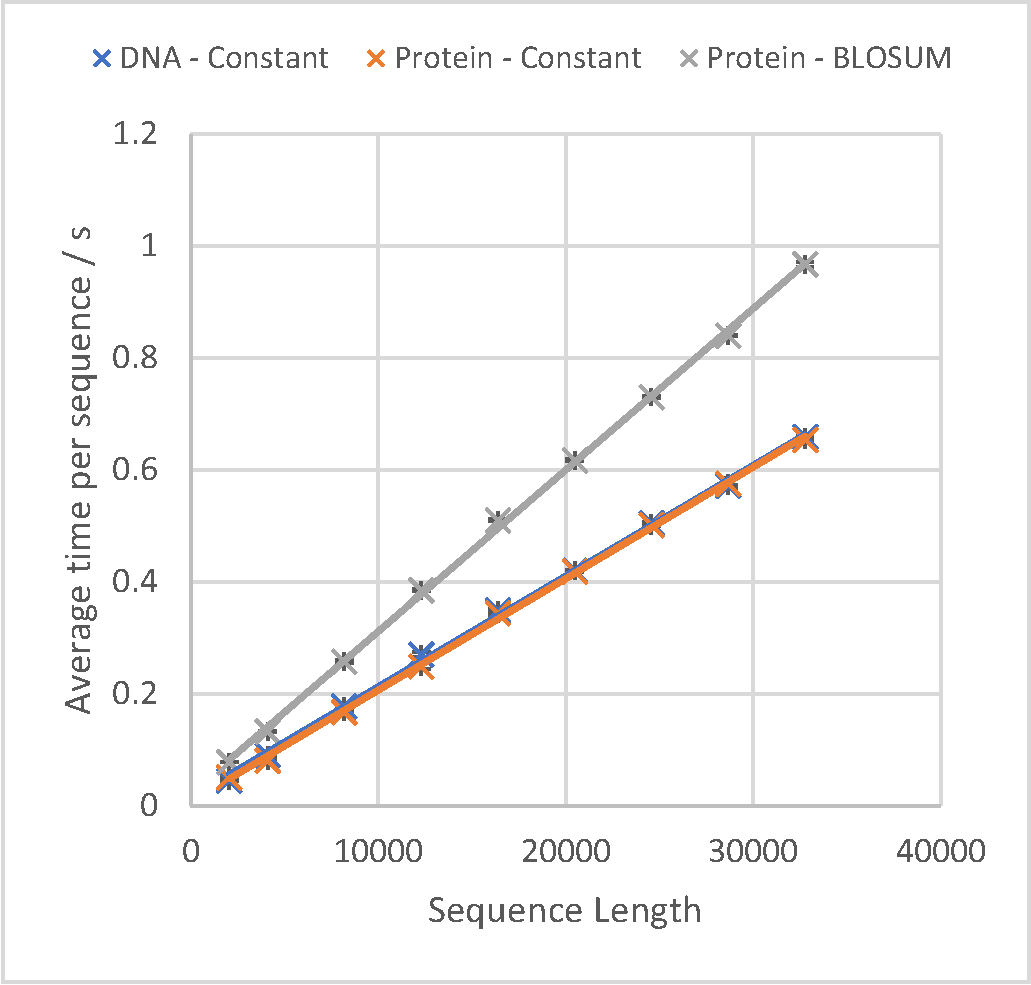
\includegraphics[width=\linewidth]{figs/eval/cu_similarity_f.pdf}
      \caption{Latency, using different similarity functions. DNA: $R^2=0.9998$, Constant~protein:~${R^2=0.9996}$, BLOSUM:~${R^2=0.9996}$}
      \label{fig:C_similarity_fun}
    \end{subfigure}
    \hfill
    \begin{subfigure}{.49\textwidth}
      \centering
      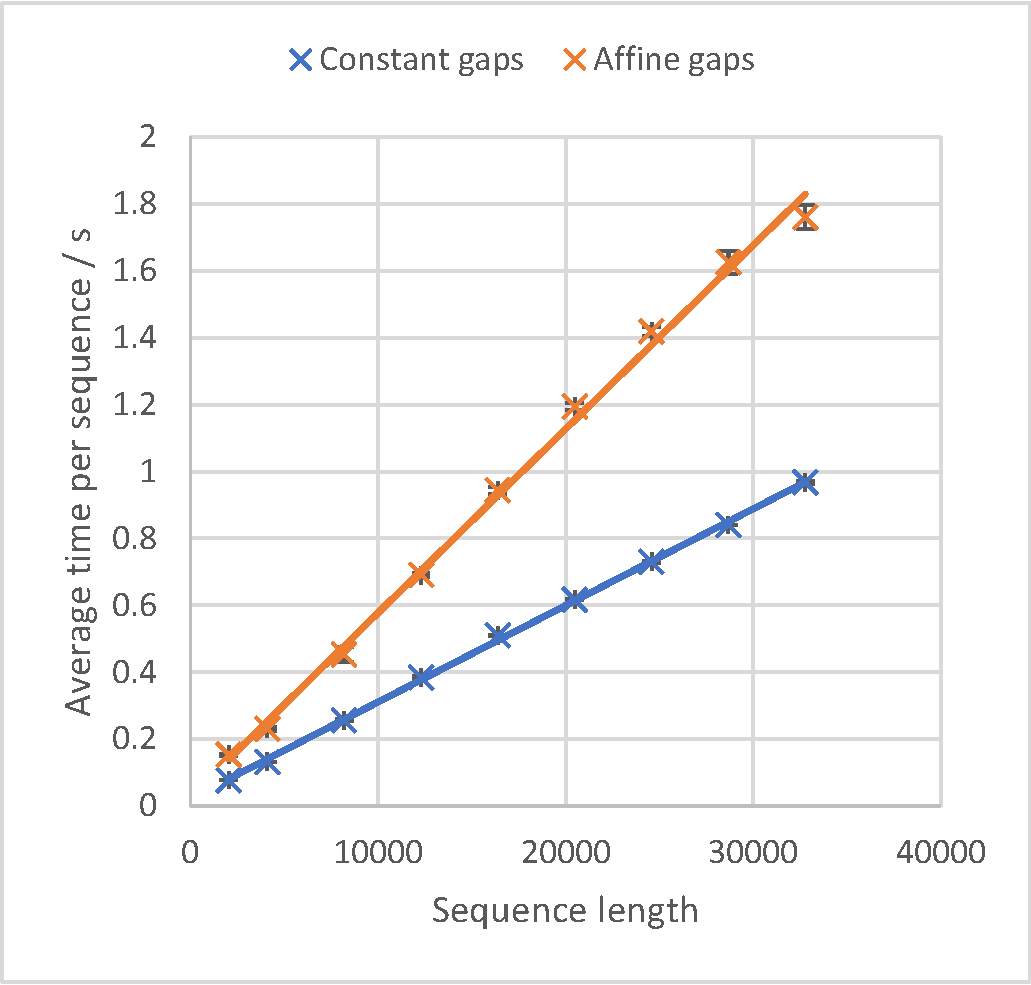
\includegraphics[width=\linewidth]{figs/eval/cu_gotoh.pdf}
      \caption{Latency using BLOSUM, using either constant or affine gaps. Constant: $R^2=0.9995$, \mbox{affine}~${R^2=0.9967}$}
      \label{fig:C_Gotoh}
    \end{subfigure}
    \caption{Latency of aligning two sequences of length $\SI{32768}{}$ against the given length, using different scoring mechanisms}
    \label{fig:C_Scoring}
\end{figure}

\subsubsection{Function occupancy}
\label{sec:C_occupancy}

I used Gprof to profile my C implementation and finding where time was spent during execution.
Gprof works by stopping the program every $\SI{0.01}{\s}$ and recording which function is being run at that time, to estimate the proportion of time spent in each function, $t$.
I profiled the alignment of a pair of sequences of lengths $\SI{32768}{}$ symbols and repeated this $10$ times.
The average function occupancy for quadratic space implementation can be found in \cref{tab:C_Quadratic_Occupancy}.

Memory access latency for the dynamic programming grid is counted in \lstinline{sw}, and for the sequence similarity matrix in \lstinline{matchBlosum}, and \lstinline{decideCell} is purely arithmetic, so there is a relatively even split between delays for arithmetic and for memory transactions.
The time taken for back-tracing was immeasurably small compared to the rest of the program.

\begin{table}
    \centering
    \begin{tabular}{|p{0.16\textwidth}|p{0.52\textwidth}p{0.08\textwidth}p{0.12\textwidth}|} \hline
        Function name & Description & Mean $t$ & Std. dev. $t$ \\ \hline
        {\ttfamily sw} & The top-level function which aligns sequences in quadratic space. & $47.23\%$ & $\pm0.886\%$ \\ \hline
        {\ttfamily decideCell} & Chooses the maximum of four scores, also returning a direction for the pointer grid, called by {\ttfamily sw}. & $42.61\%$ & $\pm1.45\%$ \\ \hline
        {\ttfamily matchBlosum} & The sequence similarity function, called by {\ttfamily sw}. & $10.16\%$ & $\pm0.983\%$ \\ \hline
        {\ttfamily backtrace} & Back-tracing routine & $0.000\%$ & $\pm0.000\%$ \\ \hline
    \end{tabular}

    \caption{Average function occupancy for quadratic space implementation in C}
    \label{tab:C_Quadratic_Occupancy}
\end{table}

The Gprof results for multi-threaded, linear space implementation were measured in a similar way and are summarised in \cref{tab:C_Linear_Occupancy}.
The quadratic space implementation was only used for a very small fraction of the time, with most of the time spent in the linear space function, or the two helper functions called by the linear space function.

\begin{table}
    \centering
    \begin{tabular}{|p{0.16\textwidth}|p{0.52\textwidth}p{0.08\textwidth}p{0.12\textwidth}|} \hline
        Function name & Description & Mean $t$ & Std. dev. $t$ \\ \hline
        {\ttfamily swLinear} & The top-level function which produces the middle column of scores using linear space, to decide how to subdivide the problem. This proportion does not include time spent in functions it calls. & $23.85\%$ & $\pm3.98\%$ \\ \hline
        {\ttfamily decideCell} & Chooses the maximum of four scores, called by {\ttfamily swLinear}. & $58.14\%$ & $\pm3.54\%$ \\ \hline
        {\ttfamily matchBlosum} & The sequence similarity function, called by {\ttfamily swLinear}. & $17.24\%$ & $\pm1.25\%$ \\ \hline
        {\ttfamily sw} & Quadratic space alignment function, called by {\ttfamily swLinear}. & $0.772\%$ & $\pm0.181\%$\\ \hline
        {\ttfamily backtrace} & Back-tracing routine for the quadratic space function. & $0.000\%$ & $\pm0.000\%$ \\ \hline
    \end{tabular}

    \caption{Average function occupancy for linear space implementation in C}
    \label{tab:C_Linear_Occupancy}
\end{table}

\subsection{CUDA implementation}
\label{sec:CUDA_eval}

\subsubsection{Setting implementation parameters}
\label{sec:CUDA_params_eval}

Like the C implementation (\cref{sec:C_params_eval}), some tuning parameters needed to be set before the CUDA implementation could be evaluated.
The first of which was the crossover point between quadratic and linear space algorithms, as discussed in \cref{sec:C_params_eval}, and is explored in \cref{fig:CU_Crossover}.
The quadratic space implementation can utilise more streaming multiprocessors as the sequences get longer, leading to stepped decreases as crossover increases.
However, large quadratic alignments can fully utilise the GPU so the graph plateaus, and GPU memory usage increases as longer sequences are aligned using quadratic space, so I set the crossover at $5120$ symbols.

\begin{figure}
    \centering
    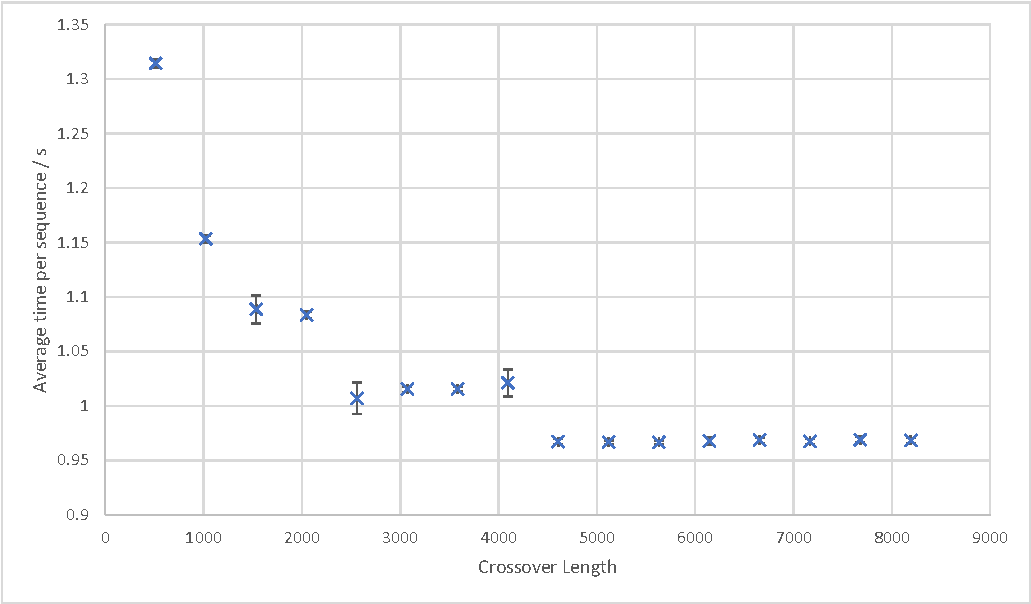
\includegraphics[width=\textwidth]{figs/eval/cu_crossover.pdf}
    \caption{Throughput of aligning two proteins both of length $\SI{32768}{}$, using BLOSUM, at different crossover points.}
    \label{fig:CU_Crossover}
\end{figure}

Also, the number of concurrent alignments needed to be decided, when measuring throughput.
To decide this, $24$ alignments were divided between different numbers of current threads, and the overall runtime is shown in \cref{fig:CU_Cores}.
The 12-thread version would not run due to the GPU running out of memory, and the figure shows that with $2$ or more threads there is a similar runtime, so two threads can produce enough work to fully utilise the GPU's resources.

\begin{figure}
    \centering
    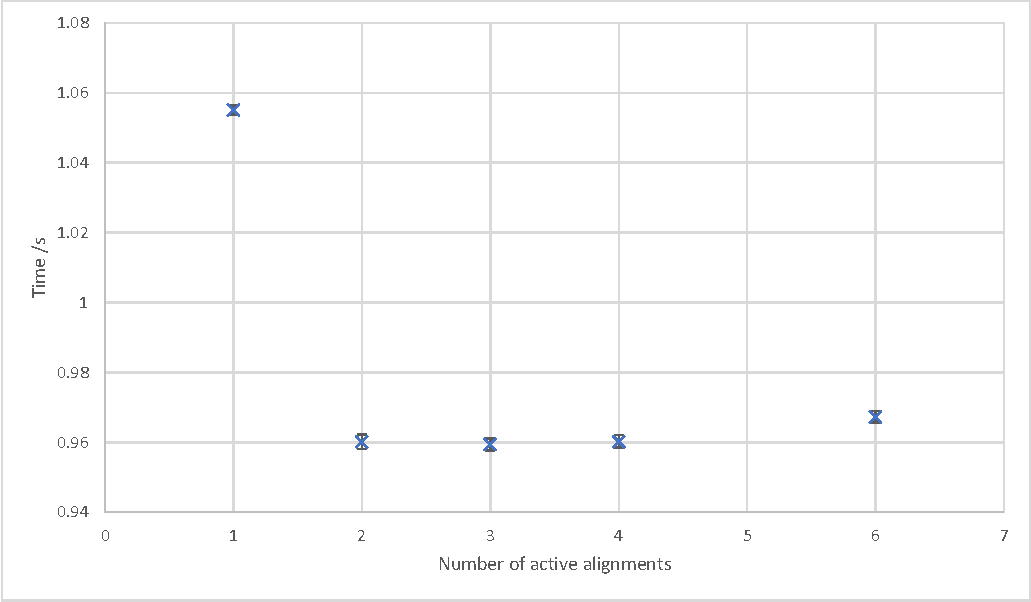
\includegraphics[width=\textwidth]{figs/eval/cu_cores.pdf}
    \caption{Time taken to aligning $24$ pairs of proteins both of length $\SI{32768}{}$, using BLOSUM, using different numbers of threads}
    \label{fig:CU_Cores}
\end{figure}

\subsubsection{Early and improved Quadratic Space implementations}
\label{sec:CUDA_single_multi_block_eval}

My initial quadratic space implementation only used one thread block, and I modified it to use more than one thread block to improve performance.
\cref{sec:Block_Parallelism_in_CUDA} contains the implementation details, and \cref{fig:CU_Multiblock} shows the difference in latency.

\begin{figure}
    \centering
    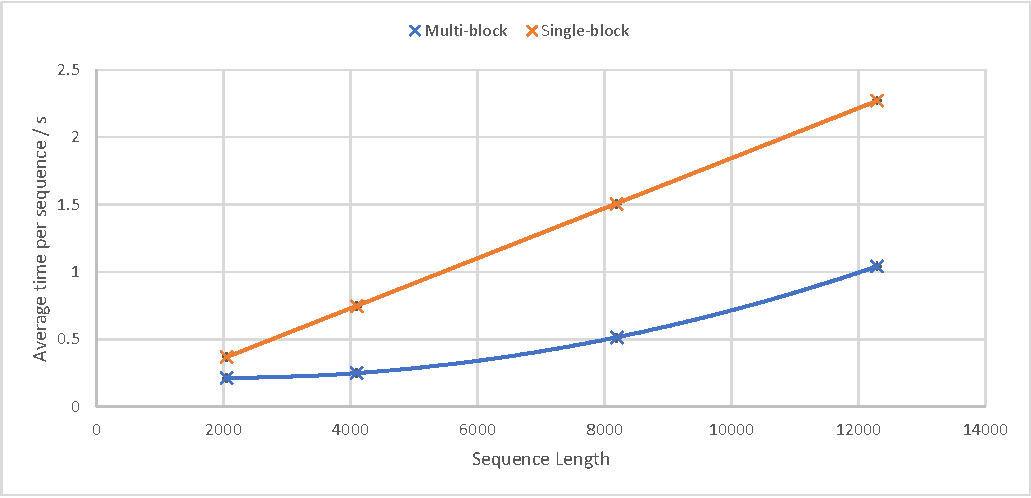
\includegraphics[width=\textwidth]{figs/eval/cu_single_block.pdf}
    \caption{Latency of aligning two proteins of length $\SI{32768}{}$ against the given length, using BLOSUM, the quadratic space algorithm. Multi-block trendline is quadratic, both $R^2=1.0000$}
    \label{fig:CU_Multiblock}
\end{figure}

\subsubsection{Quadratic and Linear Space implementations}
\label{sec:CUDA impls. eval}

Like the C implementation (\cref{sec:C_impls_eval}), latency and throughput are two helpful ways to compare the quadratic and linear space approaches.
\Cref{fig:CU_Spaces_Ser} shows the throughput of the different approaches, and the quadratic variant runs out of space after aligning sequences of lengths $\SI{32768}{}$ and $\SI{12288}{}$.
The decreasing throughput for longer sequences under the quadratic space variant is likely due to increased memory usage, so more time is spent on memory operations.
This is similar for latency (\cref{fig:CU_Spaces_Ser}).

There is a constant $\SI{86}{\milli\s}$ difference between throughput and latency for the linear space implementation, because the GPU cannot be fully utilised at the start and end of alignments, so these small amounts of idle time can be used by running two alignments at the same time.

\begin{figure}
    \centering
    \begin{subfigure}{.49\textwidth}
      \centering
      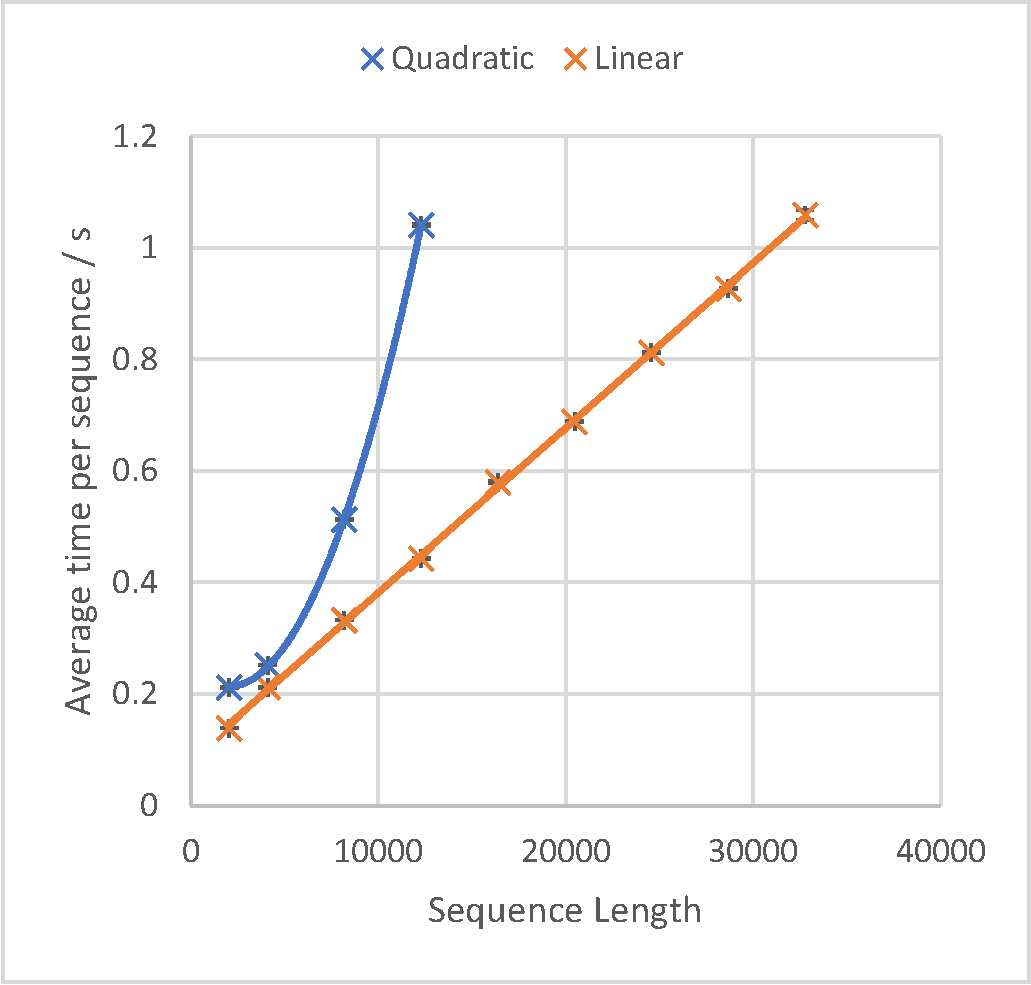
\includegraphics[width=\linewidth]{figs/eval/cu_spaces_ser.pdf}
      \caption{Latency. Quadratic: $R^2=1.000$, \mbox{Linear}:~${R^2=0.9996}$}
      \label{fig:CU_Spaces_Ser}
    \end{subfigure}
    \hfill
    \begin{subfigure}{.49\textwidth}
      \centering
      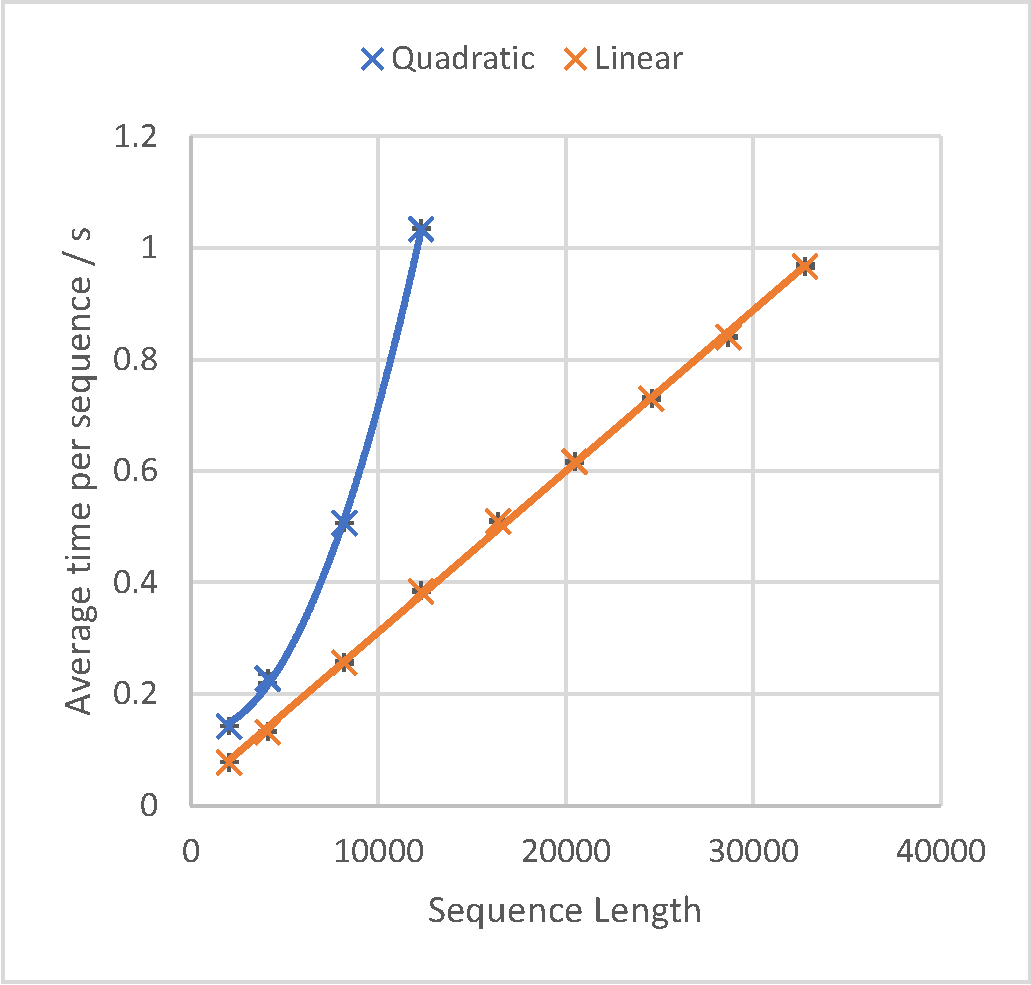
\includegraphics[width=\linewidth]{figs/eval/cu_spaces_il.pdf}
      \caption{Throughput. Quadratic: $R^2=0.9995$, \mbox{Linear}:~${R^2=0.9994}$}
      \label{fig:CU_Spaces_IL}
    \end{subfigure}
    \caption{Aligning two proteins of length $\SI{32768}{}$ against the given length, using BLOSUM, using different CUDA implementations. Quadratic has a quadratic trendline.}
    \label{fig:CU_Spaces}
\end{figure}

\subsubsection{Sequence similarity functions and scoring gaps}
\label{sec:CUDA_scoring_eval}

Similar to the C implementation, different scoring methods (\cref{sec:SW_Scoring}) were investigated.
The impact of using different sequence similarity functions is shown in \cref{fig:CU_similarity_fun}, with a significant difference between using a constant function and a lookup matrix like BLOSUM50.
There was no difference between the DNA and Protein constant functions, which unsurprising because the only thing that is different is the sequence alphabet.
However, there was a more pronounced difference in the C implementation (\cref{sec:C_scoring_eval}).

There was a significant performance penalty for using affine gaps rather than constant gaps, shown in \cref{fig:CU_Gotoh}, consistent with the additional arithmetic and memory required by affine gaps.

\begin{figure}
    \centering
    \begin{subfigure}{.49\textwidth}
      \centering
      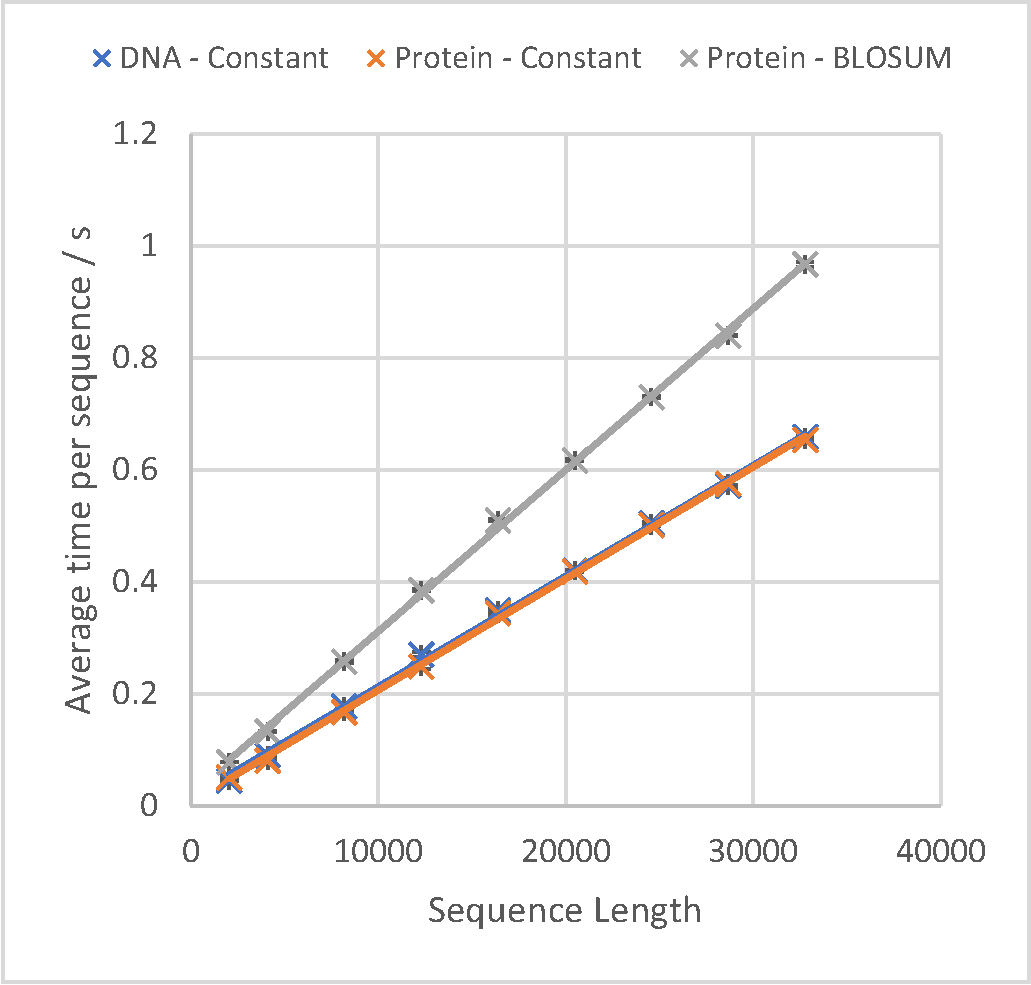
\includegraphics[width=\linewidth]{figs/eval/cu_similarity_f.pdf}
      \caption{Throughput, using different similarity functions. DNA: $R^2=0.9985$, Constant~protein:~${R^2=0.9993}$, BLOSUM:~${R^2=0.9994}$}
      \label{fig:CU_similarity_fun}
    \end{subfigure}
    \hfill
    \begin{subfigure}{.49\textwidth}
      \centering
      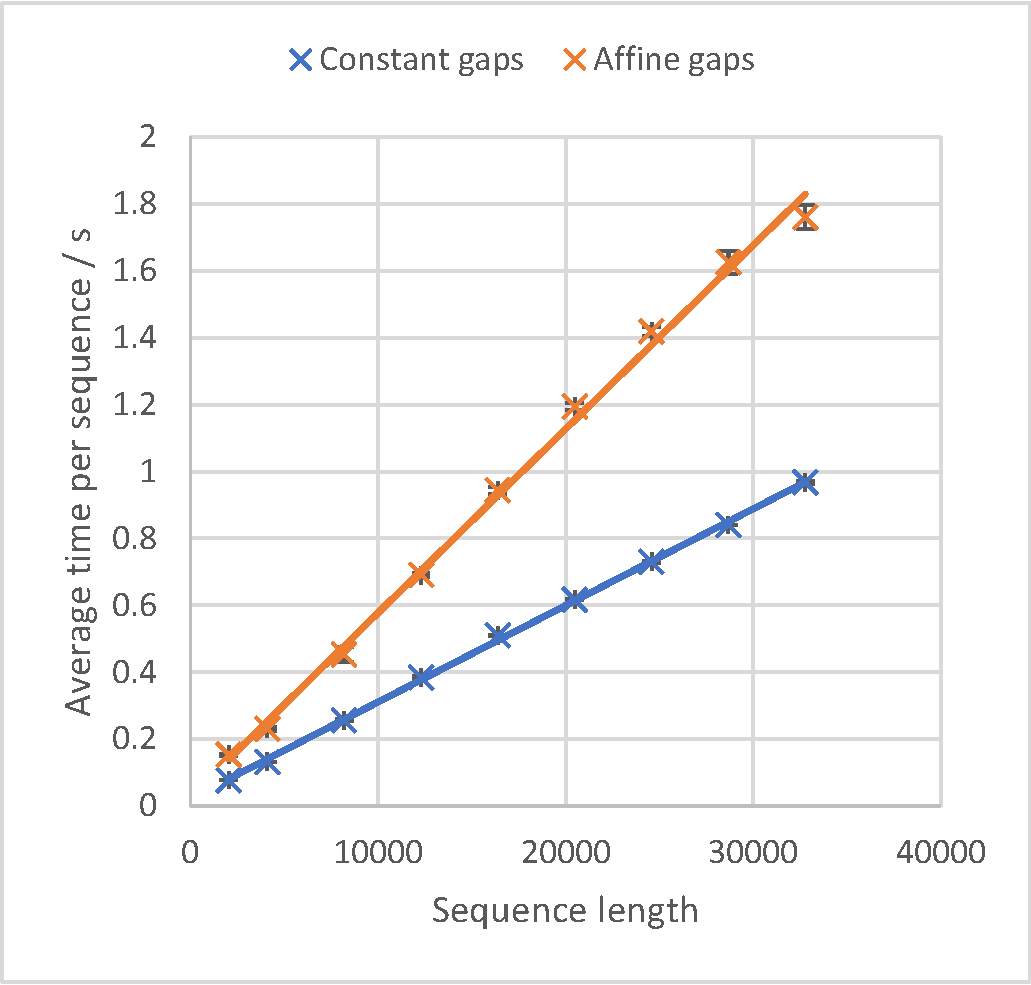
\includegraphics[width=\linewidth]{figs/eval/cu_gotoh.pdf}
      \caption{Throughput using BLOSUM, using either constant or affine gaps. Constant: $R^2=0.9994$, \mbox{affine}~${R^2=0.9964}$}
      \label{fig:CU_Gotoh}
    \end{subfigure}
    \caption{Throughput of aligning two sequences of length $\SI{32768}{}$ against the given length, using different scoring mechanisms}
    \label{fig:CU_Scoring}
\end{figure}

\subsubsection{Kernel occupancy}
\label{sec:CUDA_occupancy}
The time spent executing each kernel in a program can be measured using NVProf.
The results of using the quadratic space algorithm to produce $30$ alignments of lengths $\SI{12288}{}$ sequentially is shown in \cref{tab:CUDA_Quadratic_Occupancy}.
The alignment grid almost fills the whole GPU device memory.
The main kernel, \lstinline{sw_device}, is called multiple times for each alignment due to the way the problem is parallelised (\cref{sec:Block_Parallelism_in_CUDA}).
Back-tracing through the grid of pointers takes $5.41\%$ of execution time, whereas the C implementation spends an immeasurably small amount of time back-tracing (\cref{sec:C_occupancy}).
Moving the results from the GPU (the `device') to main memory is done by the back-tracing kernel, back-tracing is sequential so is slower on a GPU than a CPU, and filling the grid can be more effectively parallelised by the GPU.
Together this explains why back-tracing takes a larger proportion of time on the GPU than the CPU.

\begin{table}
    \centering
    \begin{tabular}{|p{0.18\textwidth}|p{0.09\textwidth}p{0.1\textwidth}p{0.105\textwidth}p{0.115\textwidth}p{0.08\textwidth}p{0.12\textwidth}|} \hline
        Name & Number of calls & Average time & Minimum time & Maximum time & Total time  & Total time prop. \\ \hline
        {\ttfamily sw} & $690$ & $\SI{12.1}{\milli\s}$ & $\SI{5.72}{\milli\s}$ & $\SI{31.1}{\milli\s}$ & $\SI{8.326}{\s}$ & $91.61\%$ \\
        {\ttfamily backtracer} & $30$ & $\SI{16.4}{\milli\s}$ & $\SI{16.3}{\milli\s}$ & $\SI{16.5}{\milli\s}$ & $\SI{491}{\milli\s}$ & $5.41\%$ \\
        CUDA {\ttfamily memcpy} Host to Device & $60$ & $\SI{4.50}{\milli\s}$ & $\SI{3.07}{\micro\s}$ & $\SI{9.33}{\milli\s}$ & $\SI{270}{\milli\s}$ & $2.97\%$ \\ \hline
    \end{tabular}

    \caption{Average function occupancy for quadratic space implementation in CUDA}
    \label{tab:CUDA_Quadratic_Occupancy}
\end{table}

The results of using the linear space algorithm to produce $30$ alignments of lengths $\SI{32768}{}$ sequentially are shown in \cref{tab:CUDA_Linear_Occupancy}.
This utilises the linear space improvements, for they are much larger than the crossover point of $5120$ (\cref{sec:CUDA_params_eval}), unlike aligning sequences of lengths $\SI{12288}{}$ as in \cref{tab:CUDA_Quadratic_Occupancy}.
My use of C++ templates results in two entries for each kernel evaluating grid cells, one for the alignments starting from the top-left ($1$), and the other when alignments can start from anywhere ($0$).
A similar proportion of time is spent back-tracing and \lstinline{addAndMaximise} is adds the two middle columns together and finds the maximum cell.

\begin{table}
    \centering
    \begin{tabular}{|p{0.18\textwidth}|p{0.09\textwidth}p{0.1\textwidth}p{0.105\textwidth}p{0.115\textwidth}p{0.08\textwidth}p{0.12\textwidth}|} \hline
        Name & Number of calls & Average time & Minimum time & Maximum time & Total time  & Total time prop. \\ \hline
        {\ttfamily swLinear\textless0\textgreater} & $1640$ & $\SI{4.51}{\milli\s}$ & $\SI{1.03}{\milli\s}$   & $\SI{7.12}{\milli\s}$ & $\SI{7.403}{\s}$ & $44.63\%$ \\
        {\ttfamily swLinear\textless1\textgreater} & $1180$ & $\SI{3.19}{\milli\s}$ & $\SI{939}{\micro\s}$ & $\SI{6.49}{\milli\s}$ & $\SI{3.770}{\s}$ & $22.73\%$ \\
        {\ttfamily swQuadratic\textless0\textgreater} & $80$ & $\SI{8.29}{\milli\s}$ & $\SI{1.16}{\milli\s}$ & $\SI{18.9}{\milli\s}$ & $\SI{663}{\milli\s}$ & $4.00\%$ \\
        {\ttfamily swQuadratic\textless1\textgreater}& $540$ & $\SI{7.12}{\milli\s}$ & $\SI{941}{\micro\s}$ & $\SI{15.2}{\milli\s}$ & $\SI{3.845}{\s}$ & $23.18\%$ \\
        {\ttfamily backtraceRunner} & $80$ & $\SI{11.2}{\milli\s}$ & $\SI{5.51}{\milli\s}$ & $\SI{24.7}{\milli\s}$ & $\SI{899}{\milli\s}$ & $5.42\%$ \\
        {\ttfamily addAndMaximise} & $70$ & $\SI{83.6}{\micro\s}$ & $\SI{6.46}{\micro\s}$ & $\SI{125}{\micro\s}$ & $\SI{5.85}{\milli\s}$ & $0.04\%$ \\
        CUDA {\ttfamily memcpy} Host to Device & $20$ & $\SI{80.8}{\micro\s}$ & $\SI{4.70}{\micro\s}$ & $\SI{195}{\micro\s}$ & $\SI{1.62}{\milli\s}$ & $0.01\%$ \\ \hline
    \end{tabular}

    \caption{Average function occupancy for linear space implementation in CUDA}
    \label{tab:CUDA_Linear_Occupancy}
\end{table}

\subsection{SystemVerilog implementation}
\label{sec:SV_eval}

\subsubsection{Expected and actual performance}
\label{sec:SV_expected_v_actual}

Using the expression derived in the \cref{sec:Processing_time_on_FPGA} it is possible to model the performance of the SystemVerilog design.
However, this does not account for issuing and collecting work from the FPGA, so performance is slightly lower in practice.
The modelled values were smaller than the measured performance (shown in \Cref{fig:FPGA_All}), and this difference is proportional to sequence length, for longer sequences will be copied to and from the FPGA.
The difference in performance between proteins (using BLOSUM) and DNA (using a constant similarity function) is due to the difference in clock speeds for their designs, $\SI{60}{\mega\hertz}$ for BLOSUM and $\SI{79}{\mega\hertz}$ for DNA.

\begin{figure}
    \centering
    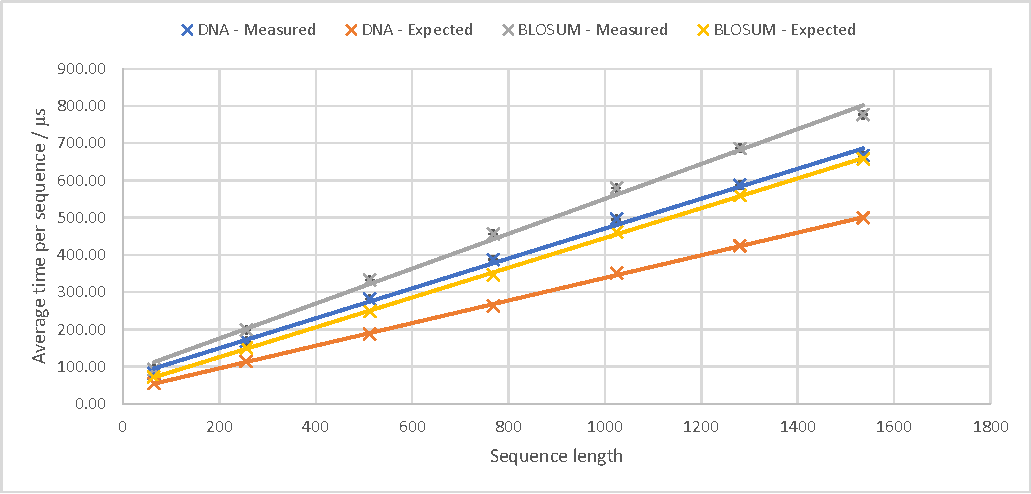
\includegraphics[width=\textwidth]{figs/eval/fpga_all.pdf}
    \caption{Modelled and actual latency of aligning two sequences of length $\SI{32768}{}$ against the given length, using a constant similarity function for DNA, and the BLOSUM50 scoring matrix for proteins. DNA: $R^2=0.9967$, BLOSUM: $R^2=0.9957$}
    \label{fig:FPGA_All}
\end{figure}

\subsubsection{Device utilisation}
\label{sec:FPGA_utilisation}

The utilisation statistics of different FPGA resources by designs help to quantify the limiting factors of the design; listed in \cref{tab:FPGA_Utilisation}.
The design aligning DNA sequences used a constant sequence similarity function, and the design aligning proteins used the BLOSUM50 lookup matrix.
Both designs use $98\%$ of the M10K blocks of RAM on the chip.
This is the limiting factor for the lengths of sequences that can be aligned, because the grid of alignment pointers are stored in block RAMs in my design.

The BLOSUM design has higher register and logic utilisation, due to the additional bits required to represent amino acids ($\SI{5}{\bits}$) rather than nucleotides ($\SI{2}{\bits}$) and the BLOSUM lookup matrix used by each processing element.
For both designs, the logic utilisation is enough to prevent the number of processing elements from being increased, as discussed in \cref{sec:Memory_in_SV}.
DSP blocks were not used, and the interconnect usage was low enough to not cause any issues.

\begin{table}
    \centering
    \begin{tabular}{|p{0.3\textwidth}|p{0.35\textwidth}p{0.35\textwidth}|} \hline
        Resource & Constant similarity DNA design & BLOSUM protein design \\ \hline
        Logic utilization (in ALMs) & $\SI{19784}{} \;/\; \SI{32070}{}$ ($62\%$) & $\SI{29635}{} \;/\; \SI{32070}{}$ ($92\%$) \\
        Total registers & $\SI{19149}{} \;/\; \SI{64140}{}$ ($30\%$) & $\SI{27405}{} \;/\; \SI{64140}{}$ ($43\%$) \\
        Total M10K Blocks & $391 \;/\; 397$ ($98\%$) & $39 \;/\; 397$ ($98\%$) \\
        Total DSP Blocks & $0 \;/\; 87$ & $0 \;/\; 87$ \\
        Average interconnect usage & $19.0\%$ & $29.0\%$ \\
        Peak interconnect usage & $38.5 \%$ & $44.5\%$ \\ \hline
    \end{tabular}
    \caption{Resource utilisation by the FPGA implementations}
    \label{tab:FPGA_Utilisation}
\end{table}

\begin{table}
    \centering
    \begin{tabular}{|l|ll|} \hline
        Design & PLL frequency  & Reported $F_{max}$ \\ \hline
        Constant similarity DNA & $\SI{79}{\mega\hertz}$ & $\SI{80.96}{\mega\hertz}$ \\
        BLOSUM Protein & $\SI{60}{\mega\hertz}$ & $\SI{60.99}{\mega\hertz}$ \\ \hline
    \end{tabular}
    \caption{Resource utilisation by the FPGA implementations}
    \label{tab:FPGA_Clocks}
\end{table}

\pagebreak

\Cref{fig:Chip_plan_base} shows the layout of FPGA resources used by the design aligning proteins using BLOSUM.
Logic elements are shown in blue, proportional to cell utilisation, and M10K blocks in green.
In \cref{fig:Chip_plan_array}, PEs in the systolic array are highlighted on a scale from white (start) to red (end).
The FIFO passing data between the last and first elements is shown in bright green, and the back-tracing unit in purple.
Some of the HPS-FPGA communication and logic is shown in yellow.
The other blue cells contain the logic and registers for retrieving and storing sequences received from the HPS.

\Cref{fig:Chip_plan_routing} shows routing utilisation.
The vertical striping is routing down columns of M10K blocks, and this is most congested around the M10K blocks that are used by but not near to the systolic array.
There is another routing hotspot around the interface pins between the FPGA and HPS.
However, none of these hotspots are congested enough to cause problems.


\subsubsection{Design clock speed}
\label{sec:SV_Fmax}

Using a Phase-locked loop (PLL), I was able to increase the clock speed of the design from the 50 MHz clock that is provided to the FPGA.
In \cref{tab:FPGA_Clocks} are the clock speeds used by my design, and the reported $F_{max}$ values for these designs.
Changing the PLL frequency changes the design as a whole and has an impact on the $F_{max}$ value reported.
The frequencies in \cref{tab:FPGA_Clocks} are based on the highest PLL frequencies I found which would result in the $F_{max}$ value being greater than the PLL frequency.
If the PLL frequency were to exceed the $F_{max}$ of the design, the design is likely to be unstable when instantiated on the FPGA.

\begin{figure}[H]
    \begin{subfigure}[b]{\linewidth}
    \centering
    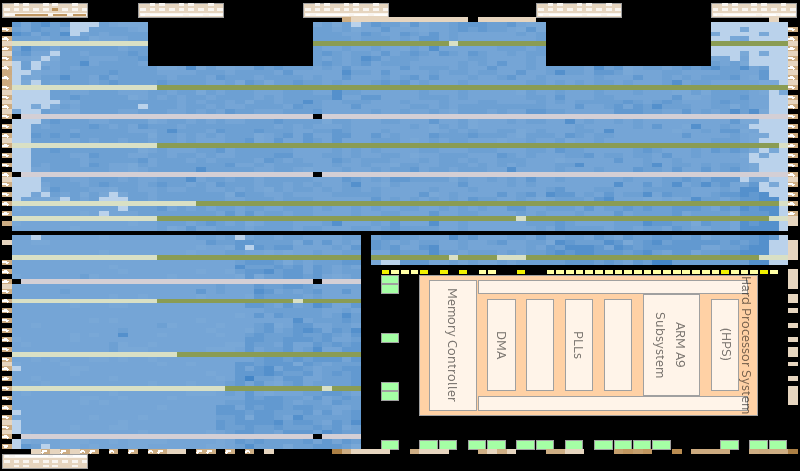
\includegraphics[width=0.72\linewidth]{figs/eval/base_chip_plan_cropped.png}
    \caption{Resources used: logic elements in blue (proportional to cell utilisation), M10K blocks in green}
    \label{fig:Chip_plan_base}
    \vspace{2ex}
    \end{subfigure}
    \begin{subfigure}[b]{\linewidth}
    \centering
    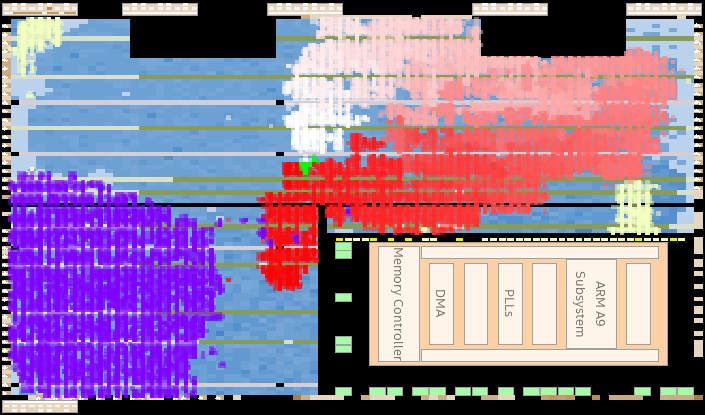
\includegraphics[width=0.72\linewidth]{figs/eval/pe_array_cropped.png}
    \caption{Different components of the design highlighted}
    \label{fig:Chip_plan_array}
    \vspace{2ex}
    \end{subfigure}
\begin{subfigure}[b]{\linewidth}
    \centering
    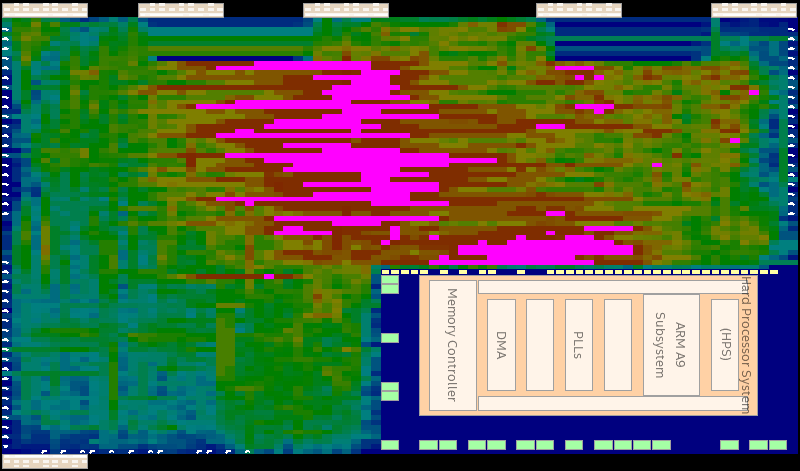
\includegraphics[width=0.72\linewidth]{figs/eval/routing_cropped.png}
    \caption{Routing utilisation, on a heatmap scale with pink for the peak areas}
    \label{fig:Chip_plan_routing}
    \vspace{2ex}
    \end{subfigure}
    \caption{FPGA chip layout of the design aligning proteins using BLOSUM}
    \label{fig:Chip_plans}
\end{figure}

